% !TEX root = ../../Diploma.tex
\section{Optimizing Parameters of a Dynamic Behaviour}
\subsection{A big network}
\subsubsection{Training}
\begin{figure}[h]
	\centering
	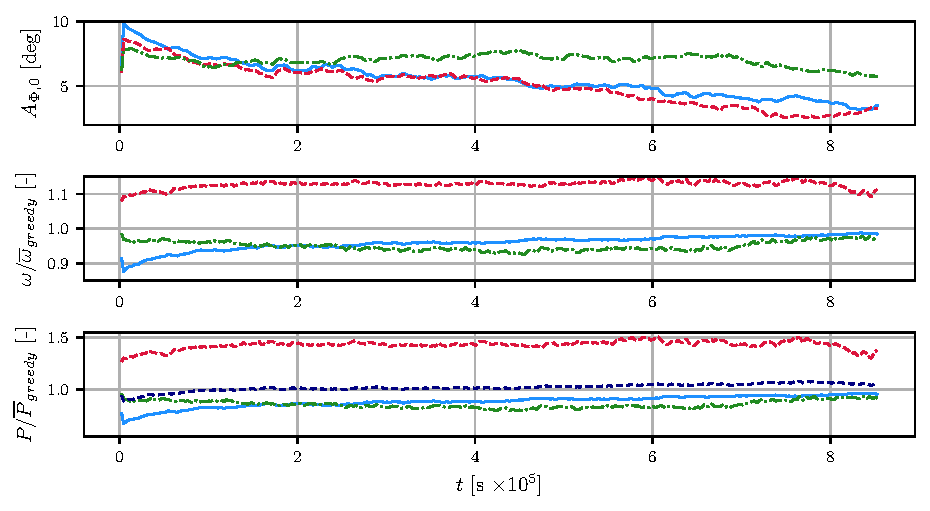
\includegraphics{parameter_optimization/DIPC_big_training.pdf}
	\caption{\legendFive{Turbine 0}{Turbine 1}{Turbine 3}{Total}{Greedy.} Training of an agent controlling the amplitude of a sinusoidal variation of the pitch according to the helix approach. Only one environment shown. All values are a rolling average with a window of width $\SI{4359}{s}$. }
	\label{fig:dipc_big_training}
\end{figure}
The time series of the training of the agent with the large network as described in \autoref{ssec:dyn_description} is shown in \autoref{fig:dipc_big_training}. It shows the amplitude of the sinusoidal signal used to control the pitch angle, the angular velocity and the power of the three turbines as well as the combined power of the park. As a benchmark the mean power generated by a park controlled by the greedy controller is also given. In the beginning the agent performs considerably worse than the benchmark. It is also visible that the amplitude changes quickly at that point, while the changes afterwards is more gradual. The figure shows a strong correlation between increase in angular velocity and generated power for each turbine, which is to be expected since the generator torque is controlled by a greedy controller. The graph shows a steady increase in total power until about $\SI{7.5e5}{s}$. At this point the power begins to decline. Again, the agent cannot remain at a local optimum. This motivates a closer look at the results and also to apply domain knowledge to judge the results and not simply accept them as optimal. \\
\begin{figure}[h]
	\centering
	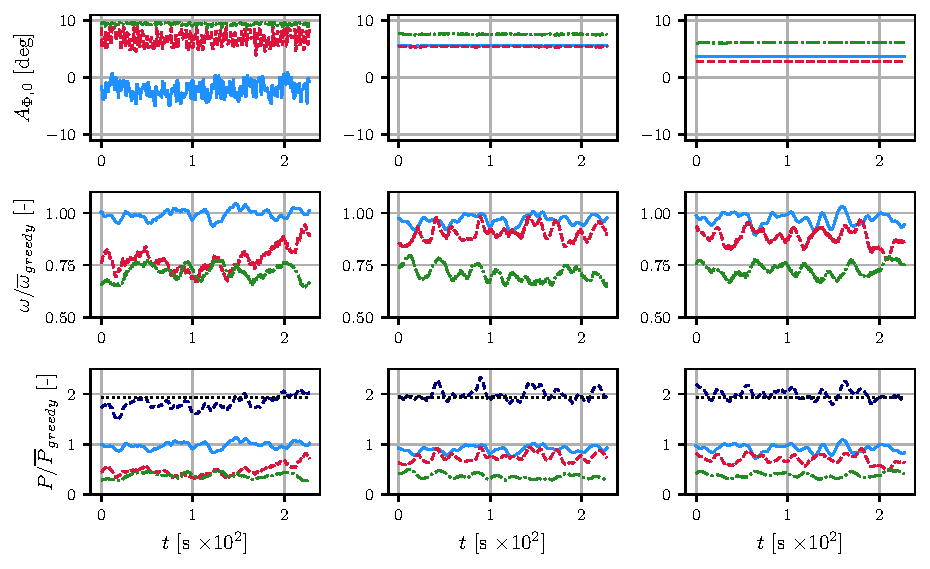
\includegraphics{parameter_optimization/DIPC_big_eval.pdf}
	\caption{\legendFive{Turbine 0}{Turbine 1}{Turbine 3}{Total}{Greedy.} Control strategy at three points during training. Left at the beginning of the training, center after half of training time, right after the training is finalized.}
	\label{fig:dipc_big_strategies}
\end{figure}
A more detailed look into the evolution of the control strategy is offered by \autoref{fig:dipc_big_strategies}. It shows the same quantities as the figure before, for one flow through time. The results in the left column are obtained with the strategy after the first update, the results in the central column with the strategy after half of the training time and the right column displays the final strategy. It shows that the initial agent reacted to the fluctuating inputs of the network, whereas the agent in the final state sets constant amplitudes. The agent after half the training time still shows some reaction, most visible in the amplitude of the last turbines pitch. That this quantity evolves the slowest can be explained by the fact, that power production is the lowest at the last turbine. Therefore the same change in relative power or $C_P$ have a lower impact on the reward. Thus the control of the last turbine evolves the slowest. The figure also shows, that the power in the last turbine has changed little over the course of the training, which is also visible in \autoref{fig:dipc_big_training}. Instead, the increase in power can be attributed to the second turbine, while the first turbine decreased in power. The strategy obtained for the last turbine is highly questionable, since curtailment of the last turbine presumably offers no benefits. Therefore a greedy strategy, that is an amplitude of zero degrees would be expected. It cannot be ruled out that this strategy would emerge with longer training. However, the computed time to reach this strategy can roughly be estimated to be $\SI{5.75e5}{s}$, when taking the mean change in amplitude over the last $\SI{1e5}{s}$. Furthermore it shows that the amplitude of the pitch of the first and the second turbine are very similar, both about four degrees. This suggests that this a good balance between optimal $C_P$ and the effects allowing for a higher power production by the following turbine.
\subsubsection{Analysis of the control strategy}
\begin{table}[h]
	\centering
	\caption{Mean, relative difference in mean and relative difference in standard deviation of power and aerodynamic moment of the helix approach after optimization in comparison to the greedy-control case.}
	\begin{tabular}{ccccccc}
	\toprule
	& \multicolumn{3}{c}{$P$}  & \multicolumn{3}{c}{$M_{aero}$ }\\ \cmidrule(rl){2-4} \cmidrule(rl){5-7}
	& mean & rel. mean & rel. std  & mean & rel. mean & rel. std \\ \midrule
	Total & $\SI{  10.4}{MW} $ & $\SI{ +6.75}{\%}$ & $\SI{ +4.78}{\%}$ &-&-&- \
	\\
	Turbine 0  & $\SI{  4.81}{MW} $ & $\SI{ -5.04}{\%}$ & $\SI{ -2.78}{\%}$ & $\SI{3.08e03}{kNm} $ & $\SI{ -3.39}{\%}$ & $\SI{ -1.14}{\%}$ \\
	Turbine 1  & $\SI{  3.67}{MW} $ & $\SI{ +43.4}{\%}$ & $\SI{ +17.6}{\%}$ & $\SI{2.57e03}{kNm} $ & $\SI{ +27.3}{\%}$ & $\SI{-0.331}{\%}$ \\
	Turbine 2  & $\SI{  1.97}{MW} $ & $\SI{ -8.95}{\%}$ & $\SI{ -12.2}{\%}$ & $\SI{1.7e03}{kNm} $ & $\SI{ -6.08}{\%}$ & $\SI{ -1.53}{\%}$ \\
	\bottomrule
	\end{tabular}
	\label{tab:dipc_big_quants}
\end{table}
To also give more quantitative results, mean as well as relative changes in mean and standard deviation of comparison to the greedy controlled case of power and aerodynamic moment are given in \autoref{tab:dipc_big_quants}. It shows that the overall gain in power is almost seven percent. It also confirms the previous observation, that this gain in power is due to an increase in power production by the second turbine, which increase by more then 40 percent. Furthermore it strengthens the assumption that the strategy of the last turbine is not optimal, since power there actually decreased by almost nine percent. Since the strategy of both previous turbines is very similar, one could expect a similar increase in power as for the second turbine. Comparing the results for the two first turbines to those obtained by Frederik et al., it can be seen that the power at the first turbine is reduced more, but that the increase in generated power at the second turbine is greater and that the overall increase in power also is considerably higher, namely $11$ percent compared to $7.5$ percent found by Frederik et al. \cite{frederik_helix_2020}. Looking beyond a simple increase in power production, quality of generated power and turbine loads are of very high importance. One measure of quality of power is low fluctuations, which is why the standard deviation of power is also given in \autoref{tab:dipc_big_quants}. It shows, that they increase in total power produced, due to a big increase in the fluctuations at the second turbine. The second aspect is the loads of the turbine, which is also a very active area of research. Therefore the analysis of loads will not be thorough, it is only pointed out, that aerodynamic torque have decreased at the first turbine and that the fluctuations have decreased at all the turbines. Therefore, like power production, the aerodynamic torque is more evenly distributed amongst the turbines, which likely has a beneficial influence on turbine lifetime. The influence on the thrust force were already assessed in \cite{frederik_helix_2020}, where only small differences compared to a greedy control were found.
\begin{figure}[h]
	\centering
	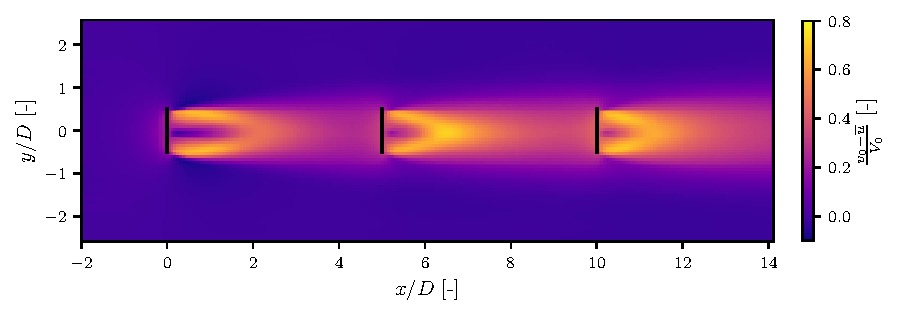
\includegraphics{parameter_optimization/DIPC_big_velocity.pdf}
	\caption{{\color{black} \rule[3pt]{22pt}{1pt} Turbine.} Mean velocity deficit compared to mean wind speed with optimized helix control.}
	\label{fig:dipc_big_vel}
\end{figure}

\begin{figure}[h]
	\centering
	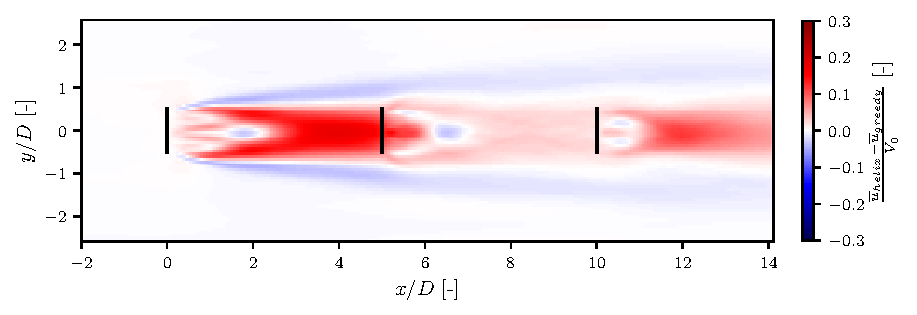
\includegraphics{parameter_optimization/DIPC_big_velocity_difference.pdf}
	\caption{{\color{black} \rule[3pt]{22pt}{1pt} Turbine.} Difference in mean velocity between optimized helix control and greedy control.}
	\label{fig:dipc_big_vel_dif}
\end{figure}
To assess the causes for the increase in power, \autoref{fig:dipc_big_vel} and \autoref{fig:dipc_big_vel_dif} show the velocity deficit in comparison to the mean wind speed and the difference in velocity in comparison to the greedy control case. As expected, a wake deficit of up to $\SI{7}{m/s}$ is visible after each turbine. Differences arise in the form of the deficit. The deficit is strongest at the tips of the blades in all cases, but at the second and the third turbine these minima meet in the center of the wake shortly behind the turbine, while they stay separated behind the first turbine. Comparing the fluid field in front of the turbine shows that the deficit in front of the third turbine is larger than in front of the second turbine. While some of the lower power production probably has to be attributed to the suboptimal control strategy, power production of the third turbine can probably not reach the amount of the second turbine since the inflow velocity is smaller. In the comparison to the greedy control case, the increased speed in the wake is brightly visible, with difference of $\SI{1.5}{m/s}$ at the core of the wake. One can also see an area of lower mean speed on the edge of the deficit. This means that the wake in the helix approach is more spread out, which is the motivation behind this approach. Behind the second turbine wind speeds are also higher, but the difference is not as big as in the first turbines wake. This is an important observation in the general behaviour of the helix approach, since Frederik et al. only considered two turbines in their study \cite{frederik_helix_2020}. If the increase in velocity can not be found after the second turbine, application to a find warm is not as beneficial as suggested by the initial study. The wake after the third turbine has again a higher velocity than in the greedy case, which again points to the fact, that more power could be generated by the third turbine.  
\begin{figure}[h]
	\centering
	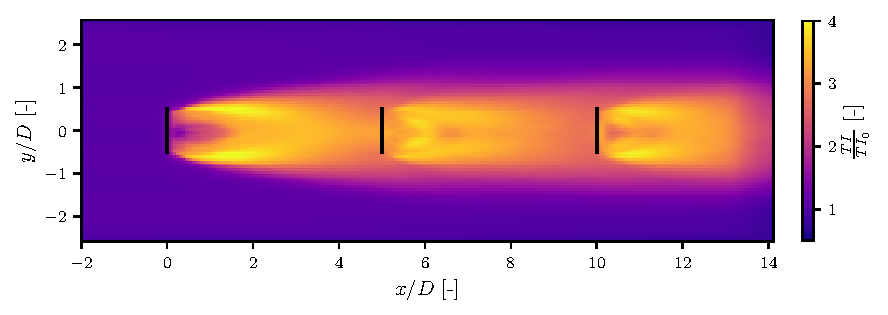
\includegraphics{parameter_optimization/DIPC_big_turbulence_intensity.pdf}
	\caption{{\color{black} \rule[3pt]{22pt}{1pt} Turbine.} Turbulence intensity of optimized helix control.}
	\label{fig:dipc_big_ti}
\end{figure} \\
\begin{figure}[h]
	\centering
	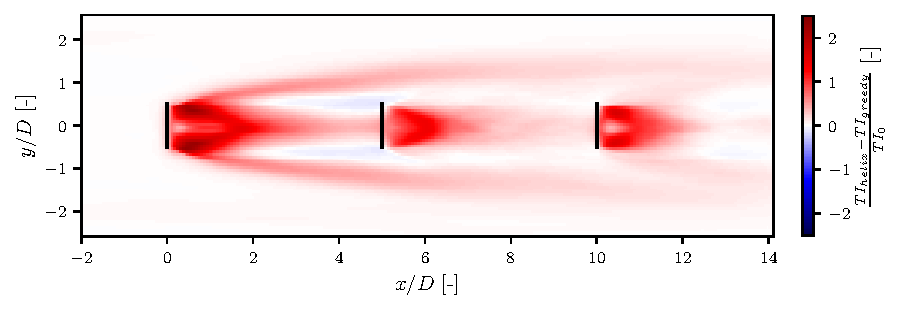
\includegraphics{parameter_optimization/DIPC_big_ti_difference.pdf}
	\caption{{\color{black} \rule[3pt]{22pt}{1pt} Turbine.} Difference in turbulence intensity between optimized helix control and greedy control.}
	\label{fig:dipc_big_ti_dif}
\end{figure} \\
The previous figures showed, that the second turbine caused a bigger wake deficit compared to inflow velocity than if it was greedy controlled. This is not the case after the first turbine, where the deficit is significantly lower. A possible explanation for this can be found in the secondary statistics of the fluid, that is its fluctuations. Therefore \autoref{fig:dipc_big_ti} shows the turbulence intensity of the helix control case and \autoref{fig:dipc_big_ti_dif} the difference of the helix control case to the greedy control case. The first figure shows that the turbulence intensity is up to four times higher in the wake. It also shows, that areas, that have a high velocity deficit, are surround by an area of high turbulence intensity. This is expected, since these are areas of high velocity gradients. Another observation that can be made is that the area with increased turbulence intensity grows in diameter up to about half a turbine distance after the second turbine and stays constant after that. A high turbulence intensity at the edges of the wake is desirable since this increases mixing of the undisturbed fluid with high momentum and fluid in the wake with less momentum. The comparison to the greedy controller shows, that this is achieved by the helix approach.\\
\begin{figure}[h]
	\centering
	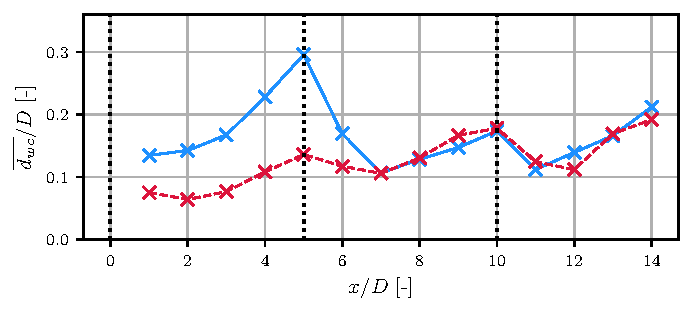
\includegraphics{parameter_optimization/DIPC_big_centers.pdf}
	\caption{\legendTwo{Helix}{Greedy}{\color{black}\rule[3pt]{1pt}{1pt} \rule[3pt]{1pt}{1pt} \rule[3pt]{1pt}{1pt} \rule[3pt]{1pt}{1pt} \rule[3pt]{1pt}{1pt} \rule[3pt]{1pt}{1pt}} Turbines. Mean distance of wake center to plane center. Crosses mark the location of the planes in which the wake center is calculated.}
	\label{fig:centers}
\end{figure}
In order to analyze the influence of the helix approach on the dynamics of the wake, the wake centers were calculated using the samwich toolbox \footnote{\url{https://github.com/ewquon/waketracking}} provided by NREL. It contains different methodologies to determine the wake center. In this work the wake center is defined as the center of a least-square fit of a Gaussian bell curve to the velocity deficit. \autoref{fig:centers} shows the distance of the wake center $d_{wc}$ to the center of the cross stream plane averaged over 100 snapshots of the fluid field at 14 planes downstream of the first turbine with a distance of a turbine diameter. It shows, that the wake is steered further away from the center after the first turbine, while this is not the case after the second turbine, where greedy and helix control lay on top of each other. After the third turbine the helix control increases the mean wake distance again. Areas, where $\overline{d_{wc}}$ is larger correspond to areas with lower mean wake deficit, which shows, that the wake is not expanded in comparison to the greedy control case, but skewed away from the center. This also explains, why a band of high turbulence intensity was visible in \autoref{fig:dipc_big_ti_dif}. This is the area only reached by the wake of the helix control case. Remarkably, the helix approach is not able to the skew the wake after the second turbine. This is most likely why the third turbine cannot increase its power production. Several aspects can contribute to this. First, the increased turbulence intensity in comparison to the inflow of the first turbine likely diffuses the tangential momentum added by the blades. Furthermore, it is questionable, whether the frequency at which the blade pitch is altered is appropriate at the second turbine. Frederik et al. showed that the wake deficit is sensitive to the Strouhal number in \cite{frederik_helix_2020}. Assuming a velocity deficit of $\SI{3}{m/s}$, the Strouhal number would increase from $\SI{0.25}{}$ to $\SI{0.35}{}$, which, according to Frederik et al., is still close to the minimal wake loss. Thus this is a possible point for future optimization, but does not account for the entire effect. However, the decreased velocity also has an effect on tangential forces exerted on the wake, since the relative velocity at the blade and the angle of attack change. Both these changes decrease the tangential force. \\
The training data showed, that the training requires a lot of computational time and that optimization is slow. However, the results did continually improve for most of the training, but, as was seen in the parameter studies as well, optimal behaviour is lost again after more training. Therefore, results of training can not be guaranteed to be optimal. The analysis of the optimized helix control showed, that due to the wake steering an increase in power production by the second turbine is possible, with little decrease in production of the first turbine. However, it also showed, that steering of the second wake was not achieved and therefore benefits for the third turbine are small, in this case even resulted in a decrease of power. Further testing of this strategy is required, for example in sheared inflow and in a park with more turbines. \\
\subsection{A small network}
\subsubsection{Training}
\begin{figure}[h]
	\centering
	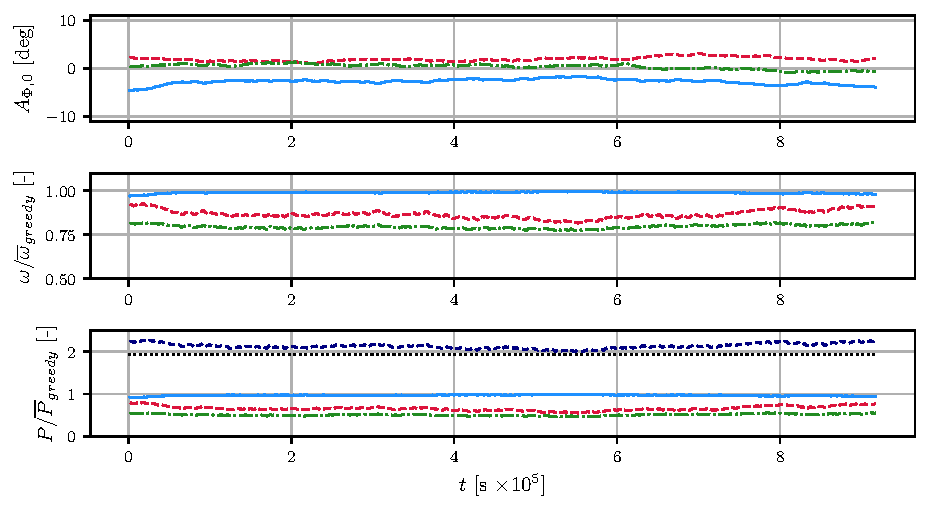
\includegraphics{parameter_optimization/DIPC_small_training.pdf}
	\caption{\legendFive{Turbine 0}{Turbine 1}{Turbine 2}{Total}{Greedy.}Training of an agent with 10 nodes per layer, controlling the amplitude of a sinusoidal variation of the pitch according to the helix approach. Only one environment shown. All values are a rolling average with a window of width $\SI{4359}{s}$.}
	\label{fig:dipc_small_training}
\end{figure}
Since the training of the agent with 400 nodes per layer proved to be computationally very expensive, a second agent with a smaller network was trained as well. The time series of the amplitude of the pitch angles, the angular velocities and generated power is shown in \autoref{fig:dipc_small_training}. It shows that the training does not reach a stable reward or action. However, the same reward and control strategy is reached twice, therefore it is assumed to be the local optimum and training is not continued further. In comparison to the agent with the larger network, training was not significantly shorter. The plots also show, that the control strategy did not change as much as during the training of the other agent and that this agent performed continuously better than the greedy-control reference.
\begin{figure}[h]
\centering
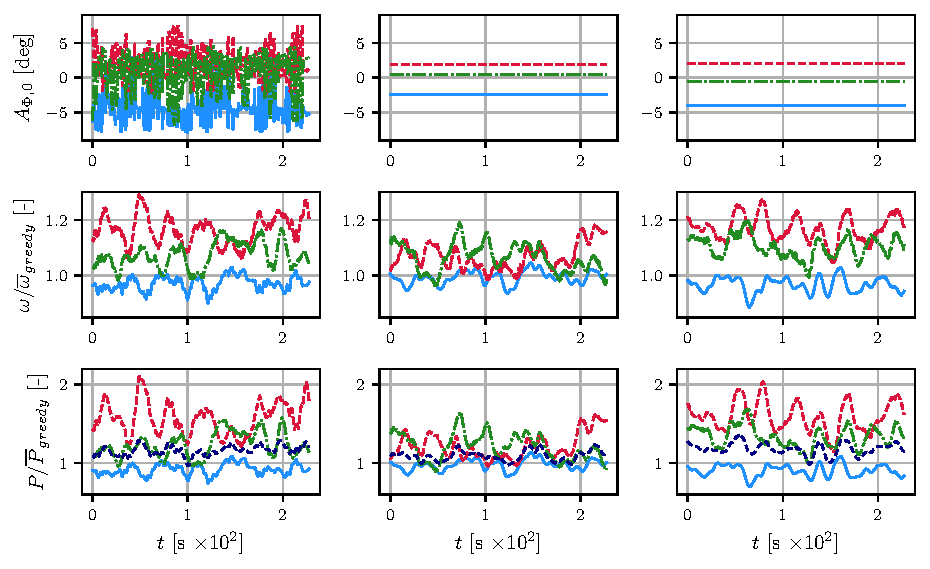
\includegraphics{parameter_optimization/DIPC_small_eval.pdf}
\caption{\legendFive{Turbine 0}{Turbine 1}{Turbine 3}{Total}{Greedy.}Control strategy at three points during training of an agent with 10 nodes per layer, controlling the parameters of a helix strategy. Left column at the beginning of the training, center column after half of training time, right column after the training is finalized.}
\label{fig:dipc_small_strategies}
\end{figure} \\
For a more detailed look at the evolution of the control strategy, \autoref{fig:dipc_small_strategies} shows the results of simulations with the agent after twelve updates, after half of the updates and in the final state. As in the previous case, in the beginning the controlled variable $A_{\Phi,0}$ varies due to a fluctuating state of the environment. After half the training, no fluctuations can be seen any more and agent prescribes a steady value for the amplitudes. The fully trained agent also sets constant values, which also only changed by a small amount in comparison to the agent after half the training. In comparison to the mean power by a greedy controlled park, the total power is always greater or equal. The strategy developed by this agent differs in two key points from that of the agent with a wider network. First, the last turbine's amplitude is close to zero, which agrees with the expected value. Second, the amplitude of the first turbine has a negative sign, which results in a phase shift of $\SI{180}{\degree}$. However, the absolute values of the amplitudes of the first and second turbine are similar between the two agents, the first agent set the amplitude of the first turbine to $\SI{3.75}{\degree}$, whereas this agent sets it to $\SI{4.0}{\degree}$. The amplitude of the second turbine differs a little more, the agent with the wide network set it to $\SI{2.85}{\degree}$ and the other to $\SI{2}{\degree}$. 
\subsubsection{Analysis of the control strategy}
\begin{table}[h]
	\centering
	\caption{Mean, relative difference in mean and relative difference in standard deviation of power and aerodynamic moment of the helix approach after optimization in comparison to the greedy-control case.}
	\begin{tabular}{ccccccc}
		\toprule
		& \multicolumn{3}{c}{$P$}  & \multicolumn{3}{c}{$M_{aero}$ }\\ \cmidrule(rl){2-4} \cmidrule(rl){5-7}
		& mean & rel. mean & rel. std  & mean & rel. mean & rel. std \\ \midrule
		Total & $\SI{  11.6}{MW} $ & $\SI{ +18.2}{\%}$ & $\SI{ +15.9}{\%}$ &-&-&- \
		\\
		Turbine 0  & $\SI{  4.76}{MW} $ & $\SI{  -5.9}{\%}$ & $\SI{  -3.9}{\%}$ & $\SI{3.06e03}{kNm} $ & $\SI{ -3.97}{\%}$ & $\SI{ -1.57}{\%}$ \\
		Turbine 1  & $\SI{  4.01}{MW} $ & $\SI{ +56.8}{\%}$ & $\SI{ +23.8}{\%}$ & $\SI{2.73e03}{kNm} $ & $\SI{ +35.1}{\%}$ & $\SI{ -2.49}{\%}$ \\
		Turbine 2  & $\SI{   2.8}{MW} $ & $\SI{ +29.0}{\%}$ & $\SI{ +13.2}{\%}$ & $\SI{2.14e03}{kNm} $ & $\SI{ +18.7}{\%}$ & $\SI{ +2.37}{\%}$ \\
		\bottomrule
	\end{tabular}
	\label{tab:dipc_small_quants}
\end{table}
The results on mean power and mean aerodynamic torque are shown in \autoref{tab:dipc_small_quants}. The overall power generated increased by $\SI{18.2}{\percent}$. This increase in total power is due to an increase of power generated by the second and the third turbine by $\SI{56.8}{\percent}$ and $\SI{29}{\percent}$, respectively. This is a bigger increase of power production by the second turbine than was reached by the other agent. The increase in power produced by the first two turbines is also twice as high as found by Frederik et al. \cite{frederik_helix_2020}. Furthermore, in the previous case the power produced by the third turbine decreased, while this time an increase is measured. That power production by the third turbine is different is to be expected since the observation was made previously, that the last turbine did not perform optimally when controlled by the other agent. However, the further increase in power produced by the second turbine is not so easily explained. Possible reasons are the phase shift between first and second turbine or the increased amplitude of the pitch oscillations of the second turbine. Power production of the first turbine decreased by almost six percent.  The aerodynamic torque of the first turbine decreased, while it increased at the other two. The dynamic load, as represented by standard deviation of $M_{aero}$, decreased for the first two turbines compared to the greedy-controlled park. It only increased at the last turbine. The decrease in dynamic loads is favourable, since dynamic loads have a negative effect on lifetime. The overall quality of power was decreased, as indicated by the standard deviation of total power. However, an increase in total power production in comparison to the decreased steadiness is probably still favourable. 
\begin{figure}[h]
	\centering
	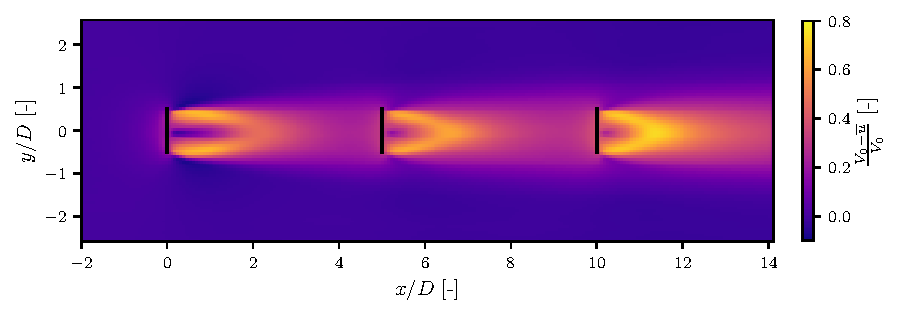
\includegraphics{parameter_optimization/DIPC_small_velocity.pdf}
	\caption{{\color{black} \rule[3pt]{22pt}{1pt} Turbine.} Mean velocity deficit compared to mean wind speed with optimized helix control.}
	\label{fig:dipc_small_vel}
\end{figure} \\
To investigate the effects of this control strategy further, the mean wake deficit of a simulation with the agent with a small network is shown in \autoref{fig:dipc_small_vel}. It shows, that the maximum wake deficit occurs after the third turbine as it is expected for optimal behaviour. Furthermore it shows that the wake deficit in front of the second and the third turbine is small, which is also expected for optimal behaviour. The comparison to the previous agent shows, that the wake deficit after the second turbine is significantly smaller, even though the power production is increased. This also causes the inflow velocity of the third turbine to be higher, which also allows for a higher power production there.
\begin{figure}[h]
	\centering
	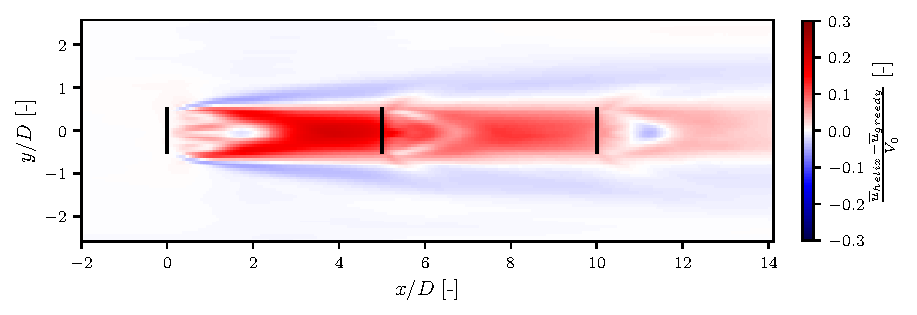
\includegraphics{parameter_optimization/DIPC_small_velocity_difference.pdf}
	\caption{{\color{black} \rule[3pt]{22pt}{1pt} Turbine.} Mean velocity when turbines are controlled with optimized helix control compared to greedy controlled case.}
	\label{fig:dipc_small_vel_diff}
\end{figure} \\
The comparison to the greedy controller in \autoref{fig:dipc_small_vel_diff} shows a similar picture. In an area about the width of one diameter the velocity behind the first and second turbine is significantly higher, further away from the center a higher velocity deficit is visible. This was also the case when the turbines were controlled by the agent with a wider network. The increase in spread of the wake is similar to the other agent. However, the wake deficits near the core of the wake differ. Behind the second turbine only a small conic shell has a higher deficit in comparison to the greedy controller, while the rest of the seconds turbine's wake has a significantly lower deficit. Behind the third turbine the velocity deficit of the turbine controlled by this agent is higher than when the park is controlled by the other agent, which is probably due to a higher oscillation amplitude. 
\begin{figure}[h]
	\centering
	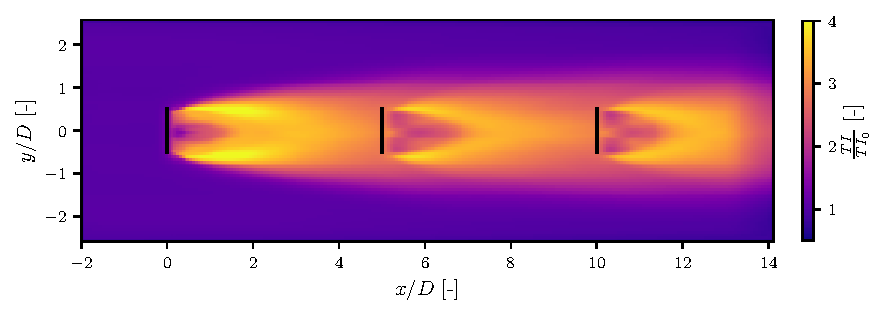
\includegraphics{parameter_optimization/DIPC_small_turbulence_intensity.pdf}
	\caption{{\color{black} \rule[3pt]{22pt}{1pt} Turbine. }Turbulence intensity of park controlled with optimized helix control compared to turbulence intensity at inlet.}
	\label{fig:dipc_small_ti}
\end{figure}\\
To show the second order statics of the flow, \autoref{fig:dipc_small_ti} shows the turbulence intensity of a park controlled by this agent. It shows that the turbulence intensity is increased in the wake, but also that an area of low increase exists behind the second and third turbine. It shows also that the highest increase in turbulence intensity is after the first turbine. The maximum of turbulence intensity in each wake decreases in stream direction. After the first, but especially after the second turbine the coss-sectional area of high turbulence intensity quickly decreases downstream. After the third turbine this is not the case, this can most likely be attributed to low pitch oscillation, but effects due to the end of domain can play a role as well. The distribution of turbulence intensity after the first turbine is very similar to that of the park controlled by the agent with a large network. This is not the case after the second and third turbine. After the second turbine the area of lower increase of $TI$ does not exist in the park controlled by the other agent. After the third turbine it is significantly smaller. Also the decreasing diameter of the area of high intensity is not visible. Therefore it must be caused by the phase shift or the increased oscillation amplitude.
\begin{figure}[h]
	\centering
	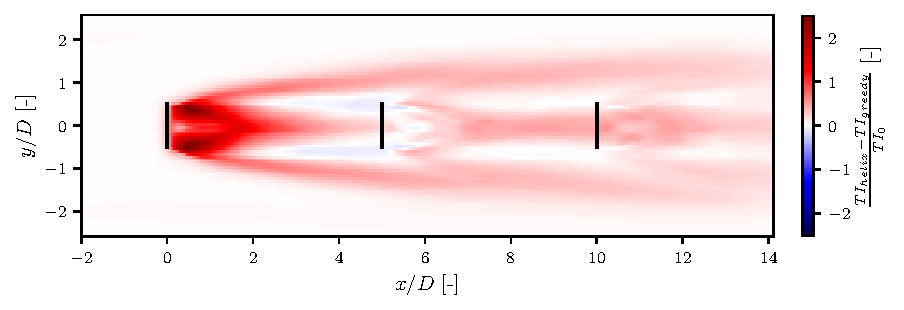
\includegraphics{parameter_optimization/DIPC_small_ti_difference.pdf}
	\caption{{\color{black} \rule[3pt]{22pt}{1pt} Turbine. }Turbulence intensity of park controlled by optimized helix control compared to greedy-controlled park.}
	\label{fig:dipc_small_ti_diff}
\end{figure}\\
In \autoref{fig:dipc_small_ti_diff} the difference in turbulence intensity in comparison to a greedy-controlled park is shown. It shows, that the turbulence intensity is increased throughout the wake with the exception of a narrow annular ring with the diameter of the turbine. This shell is visible in each wake and begins around $1.5 D$ downstream of the turbines. The difference in $TI$ is of the same magnitude in the wake of the second and third turbine. The figure also shows that an area of increased turbulence intensity exists connecting the second turbine to the outer area of turbulence intensity. Furthermore this outer area has a higher turbulence intensity compared to the park controlled by the agent with the wider network. This suggests that the wake might be steered outside the center like the wake of the first turbine. This was not the case when controlled by the other agent. This would offer an explanation of the increased velocity and consequently higher power production at the third turbine. 
\begin{figure}[h]
	\centering
	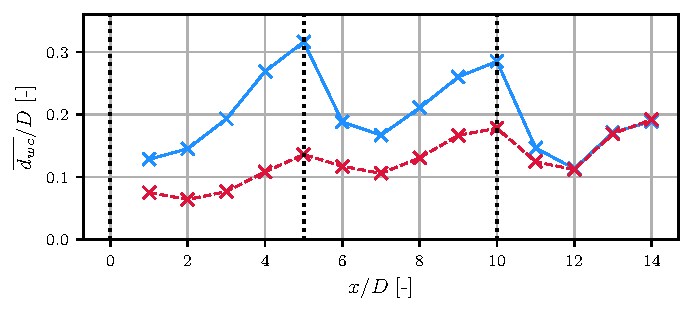
\includegraphics{parameter_optimization/DIPC_small_centers.pdf}
	\caption{\legendTwo{Helix}{Greedy.}Mean distance of wake center to center of cross-plane at 14 cross-planes.}
	\label{fig:dipc_small_centers}
\end{figure} \\
To verify this last hypothesis, the mean distance of the wake center to the center of the cross plane is shown in \autoref{fig:dipc_small_centers}. It shows again, that wake of the first turbine is steered further away from the center than if the turbine had no oscillation. The same is true for the second turbine. This confirms the previous hypothesis and explains the increased power production of the third turbine. This leads to the question why the oscillations cause the steering in this case but not in the park controlled by the other agent. Since the wake of the first turbine is the same in either case, two possible explanations remain. It is either caused by the decreased amplitude of oscillations by the second turbine or the phase shift of the oscillations at the first turbine. To test this, simulations with a controller with the same amplitudes were run, one with phase shift and one without. The mean wake distance to the cross-wise center are shown in \autoref{fig:phase_shift}. It clearly shows that the increased in $\overline{d_{wc}}$ after the second turbine is caused by the phase shift.  
\begin{figure}
	\centering
	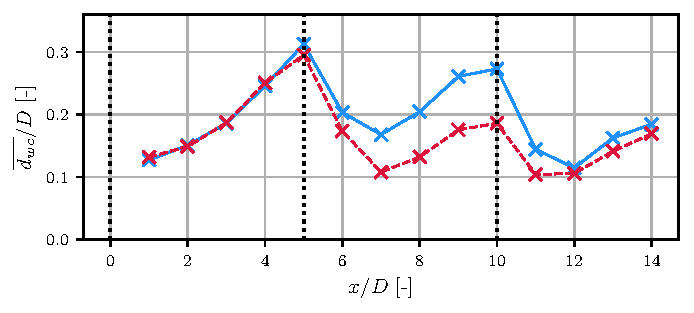
\includegraphics{parameter_optimization/Phase_shift_centers.pdf}
	\caption{\legendTwo{Phase shift}{No phase shift} Two controllers with helix control and values optimized by second agent.}
	\label{fig:phase_shift}
\end{figure}
\subsubsection{Analysis of the helix control strategy for two turbines}
To further investigate the influence of the phase shift, a look back at the governing physics has to be taken. Frederik et al. \cite{frederik_helix_2020} showed, that the oscillation of the pitch angles with the helix approach results in moments in vertical and cross-stream direction, $M_{tilt}$ and $M_{yaw}$, respectively. The resulting moment vector will be called $\vec{M}_{osc}$. They oscillate with the excitation frequency $f_e$ and with an amplitude $A_M$ :
\begin{align}
\vec{M}_{osc} &=
\begin{bmatrix}
M_{tilt}(t) \\
M_{yaw}(t)
\end{bmatrix} = 
A_M \cdot
\begin{bmatrix}
sin(2\pi f_e t) \\
\cos(2\pi f_e t)
\end{bmatrix}
\end{align}
The moment resulting on the wake after the second turbine will be called $\vec{M}_{helix,1}$. It is the sum of $\vec{M}_{osc,1}$ due to oscillations by the second turbine and the moment transported by the wake from the first turbine $\vec{M}_{helix,0}$. It is equal in magnitude to $\vec{M}_{osc,0}$ but rotated by $\phi_{travel}=2 \pi f_e T_{travel}$, since it is the moment exerted by the turbine time $T_{travel}$ ago. With $A_{M,0}$ and $A_{M,1}$ as the amplitudes of the moments exerted by the first and second turbine, respectively, and $\vec{I}$ as the identity matrix and $\vec{R}(\phi)$ as the rotation matrix about angle $\phi$, the moment of the helix after the second turbine is:
\begin{equation}
	\vec{M}_{helix,1} = \vec{M}_{osc,1} + \vec{M}_{helix,0} = \left(A_{M,1} \vec{I} + A_{M,0} \cdot \vec{R}(\phi_{travel})\right) 
	\cdot 
	\begin{bmatrix}
	\sin(2\pi f_e t) \\
	\cos(2\pi f_e t)
	\end{bmatrix} .
\end{equation}
The magnitude of the resulting moment $\vec{M}_{helix,1}$ is:
\begin{align}
	\Vert\vec{M}_{helix,1}\Vert &= \sqrt{A_{M,1}^2 + A_{M,0}^2 + 2 A_{M,0} A_{M,1} \cos(\phi_{travel})}  \label{eq:helix_moment}.
\end{align}
It shows that the previous turbine influences it in two ways. The term $A_{M,0}^2$ can not be negative and must therefore increase the moment. Only the second term, which contains the amplitude and the cosine of $\phi_{travel}$ can result in a decrease in $\vec{M}_{helix}$. Assuming that $A_{M,0}$ is proportional to $A_{\Phi,0}$, which is the amplitude of the pitch oscillations, the negative amplitude results in an increase in $\vec{M}_{helix}$ if $\cos(\phi_{travel}) < 0$. With $St$ and mean inflow velocity $V_0$, $\phi_{travel}$ is:
\begin{align}
	\phi_{travel} & = 2 \pi \mathrm{St} \frac{V_0}{V_{helix}} \frac{d_{Turbines}}{D} \label{eq:phi_travel},
\end{align} 
with $V_{helix}$ as the transportation velocity of the helix. In the case studied, $\phi_{travel} = 5\pi/2 \cdot V_0 / V_{helix}$. Since the wake cannot be faster than the inflow velocity and considering the results from \autoref{fig:dipc_small_vel}, $ 3 \geq V_0/V_{helix} \geq 1$ and therefore $\cos(\phi_{travel})  \leq 0$. Thus a negative amplitude and the resulting phase shift must be beneficial.\\
Comparing $\vec{M}_{helix,1}$ and $\vec{M}_{helix,0}$, it can be shown that the two moments have a phase shift of $\phi_0$:
\begin{equation}
	\tan(\phi_0) = \left(\frac{A_{M,0} \cos(\phi_{travel})}{A_{M,1}+ A_{M,0} \cos(\phi_{travel})}-1\right) \tan(\phi_{travel}) \label{eq:phi_0}
\end{equation}
To eliminate this phase shift in the helix, a phase shift in the oscillations at the second turbine can be introduced. Adding a phase shift of $\phi_{travel}$ to $\vec{M}_{osc,1}$ results in:
\begin{equation}
	\vec{M}_{helix,1} = \left( A_{M,1} + A_{M,0} \right) \vec{R}(\phi_{travel}) \cdot
	\begin{bmatrix}
	\sin(2\pi f_e t) \\
	\cos(2\pi f_e t)
	\end{bmatrix} .
\end{equation}
The magnitude of this new moment is easily shown to be:
\begin{equation}
 \Vert\vec{M}_{helix,1}\Vert =  A_{M,1} + A_{M,0}
\end{equation}
By design, the helix before and after the turbine do not have a phase shift. \\
To implement this phase shift, first $\phi_{travel}$ has to be found. From \eqref{eq:phi_travel} all quantities except the transportation velocity $V_{helix}$ are known. To measure this velocity, the phase angle of the wake center in each $y$-$z$-plane of the wake behind the first turbine is calculated. The mean of $\phi_{total}$ of 200 timesteps is calculated. The velocity is calculated by $V_{helix} = 2\pi f_e x/\phi_{total}$. The velocity is computed from the angles between $2.5D$ and $3.8D$, to avoid disturbances due to the turbines. In the case studied $V_{helix}/V_0 = 0.818$. The mean total angle and the angle predicted by $V_{helix}$ are shown in \autoref{fig:phi_total}. The figure shows good agreement between the two quantities in the wake after the first turbine, but significant deviation after the second turbine, which is to be expected due to the phase shift predicted by \eqref{eq:phi_0}.
\begin{figure}[h]
	\centering
	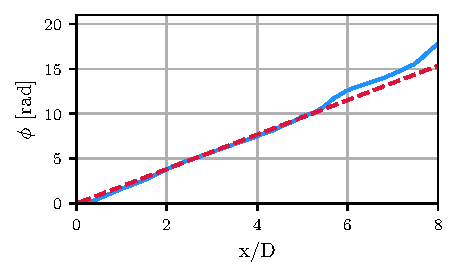
\includegraphics{parameter_optimization/phi_total.pdf}
	\caption{\legendTwo{$\overline{\phi_{total}}$}{$2 \pi f_e x / V_{helix}$}}
	\label{fig:phi_total}
\end{figure}
The measured velocity predicts a rotation of $\phi_{total}=3.06\pi$. This is very close to $3\pi$ which would be the same as a phase shift of $\pi$ as was performed by the agent. In \autoref{tab:optimal_greedy} the mean , difference in mean relative to a greedy controller and difference standard deviation relative to a greedy controller are shown for power and $M_{aero}$. A comparison to \autoref{tab:dipc_small_quants} shows that the two are almost equivalent, differences are in the range of five percent for most quantities.
\begin{table}[h]
	\centering
	\caption{Mean and relative difference in mean and standard deviation to a greedy control case of power and aerodynamic moment of a park controlled with the phase shifted helix strategy.}
	\begin{tabular}{ccccccc}
		\toprule
		& \multicolumn{3}{c}{$P$}  & \multicolumn{3}{c}{$M_{aero}$ }\\ \cmidrule(rl){2-4} \cmidrule(rl){5-7}
		& mean & rel. mean & rel. std  & mean & rel. mean & rel. std \\ \midrule
		Total & $\SI{  11.5}{MW} $ & $\SI{ +17.5}{\%}$ & $\SI{ +14.3}{\%}$ &-&-&- \
		\\
		Turbine 0  & $\SI{  4.76}{MW} $ & $\SI{ -5.88}{\%}$ & $\SI{  -5.3}{\%}$ & $\SI{3.06e03}{kNm} $ & $\SI{ -3.96}{\%}$ & $\SI{ -2.11}{\%}$ \\
		Turbine 1  & $\SI{  3.95}{MW} $ & $\SI{ +54.5}{\%}$ & $\SI{ +28.6}{\%}$ & $\SI{2.7e03}{kNm} $ & $\SI{ +33.8}{\%}$ & $\SI{-0.523}{\%}$ \\
		Turbine 2  & $\SI{  2.79}{MW} $ & $\SI{ +28.6}{\%}$ & $\SI{ +12.8}{\%}$ & $\SI{2.14e03}{kNm} $ & $\SI{ +18.4}{\%}$ & $\SI{ +1.71}{\%}$ \\
		\bottomrule
	\end{tabular}
	\label{tab:optimal_greedy}
\end{table} \\
In conclusion, the phase shift in the helix arriving at the second turbine explains why a helix exists after the second turbine, when the park is controlled by the second agent, but not when it is controlled by the first agent. It also explains the increase in power produced by the second turbine when controlled by the second agent in comparison to the control strategy developed by the first agent, since the smaller wake deficit after the second turbine leads to a smaller induced velocity at the second turbine. From a more general perspective, the results presented in this chapter showed, that the agent is able to improve its behaviour. Furthermore it showed how reinforcement learning can be a valuable tool for scientific research, as it might find strategies not thought of by individual researchers as well as the possibility to try many different strategies at once. Not only can it help discover new control strategies but in this, hint at new physical phenomena not yet considered. On the other hand, it also showed some of the limiting factors. The training, even of an agent with a small network, takes a lot of computational effort and optimality can not be guaranteed. In the field of control strategies for wind parks, it was shown that the helix control has great potential to improve total generated power. It could also be shown that this strategy can be extended to bigger wind parks by phase shifting the helices of the turbines. To further the understanding of the phenomena caused by a helical wake, a thorough assessment of the loads will have to be made as well as simulations and field tests of bigger wind parks. Additionally the influence of a sheared boundary layer has not yet been studied, which will likely have a crucial influence, as the shear also influences the wake meandering.